\section{Gyrosensor Programmierung (Koch)}
Zu Beginn des Projekts war geplant den Gyrosensor MPU6050 zu nutzen, um die Position der Geschützplattform zu bestimmen, da eine kontinuierliche Bewegung um die eigene Achse aufgrund der Kabel nicht möglich ist. Dabei sollte der Sensor über den I2C-Bus mit dem Raspberry Pi 5 verbunden werden, um die Daten auszulesen und zu verarbeiten.
Der MPU6050 ist dabei ein 3-Achsen-Gyroskop und 3-Achsen-Beschleunigungssensor, welcher entsprechende Drehbewegungen und Beschleunigungen entlang der Raumachsen messen kann, welche für eine genaue Winkelbestimmung notwendig sind.

Nach kurzem Einlesen in die Dokumentation waren erste Rohdaten leicht auszulesen. Diese Rohdaten liegen in Form von 16 Bit in zwei Registern bereit und haben die Einheit $\mathit{LSB/g}$ für die Beschleunigungswerte und $\mathit{LSB/^\circ s}$ für die Gyroskop-Werte. Dies gilt es in tatsächliche physikalische Größen umzuwandeln, was bei unserem Projekt letztlich einem Winkel entspricht. 
Um die Beschleunigungswerte nutzen zu können, muss dafür mittels des Skalierungsfaktors die Fallbeschleunigung $\mathit{g}$ errechnet werden, indem man den erhaltenen Wert $x/16384$ rechnet. Die $16384$ ergeben sich aus der Dokumentation und entsprechen den LSB bei einem Messbereich von $\pm2g$, welches der Standardauflösung entspricht und auch die höchste Auflösung des MPU6050 für ist.
Ähnlich wird nun auch Winkelgeschwindigkeit ($\mathit{^\circ s}$) errechnet. Hierbei beträgt der Teiler standardmäßig $131$. \cite[S. 12-13]{raspberry_invensense_mpu6050_datasheet} 

Nach der Umrechnung der Rohdaten in physikalische Größen können nun die Neigungswinkel (Roll- und Pitch-Winkel) des Sensors berechnet werden. Diese ergeben sich aus der Richtung der Erdbeschleunigung relativ zum Sensor. 

Dazu wird die Erweiterung des Arkustangens genutzt, genauer gesagt die Funktion \texttt{atan2}, da sie im Gegensatz zum gewöhnlichen Arctangens auch die Orientierung in allen vier Quadranten berücksichtigt und somit stabile Winkelwerte über den gesamten Bereich von $-180^\circ$ bis $+180^\circ$ liefert. \cite{raspberry_matlab_atan2}

Die Winkelberechnung erfolgt nach der Formel \ref{eq:norms_to_angle}:

\begin{gather}
    \begin{aligned}
    \varphi_\text{pitch} &= \arctan2\left(a_y,\sqrt{a_x^2 + a_z^2}\right) \cdot \frac{180^\circ}{\pi} \\
    \varphi_\text{roll}  &= \arctan2\left(a_x,\sqrt{a_y^2 + a_z^2}\right) \cdot \frac{180^\circ}{\pi}
    \end{aligned}
    \label{eq:norms_to_angle}
\end{gather}


Hierbei sind $a_x$, $a_y$ und $a_z$ die normierten Beschleunigungswerte in $\mathit{g}$ (berechnet aus den Rohwerten durch Division durch $16384$). 

Nachdem der Term im Code implementiert wurde, konnte ein starkes Rauschen beobachtet werden, was zunächst auf natürliche Schwankungen des Sensors zurückgeführt wurde, weshalb sich dazu entschieden wurde zuerst einen Komplementärfilter zu implementieren,
welcher allerdings das Problem nur bedingt beheben konnte. Deshalb wurde auch noch der Kalman-Filter ausgetestet, wodurch auch eine starke  Rauschunterdrückung festgestellt werden konnte, doch auch hier zeichnete sich ein überdurchschnittliches Rauschverhalten ab, weshalb der Fehler nicht mehr auf ein natürliches Rauschen zurückzuführen war.
Daraufhin wurde auch ein zweiter MPU6050 getestet, welcher ebenfalls dieses Verhalten aufwies, wodurch klar wurde, dass es sich hierbei um einen Programmierfehler handeln muss. Dieser konnte nach einiger Zeit auch herausgefunden werden und lag an der Interpretation der Rohdaten, 
welche fälschlicherweise als \texttt{int16\_t} statt \texttt{uint16\_t} interpretiert wurden. Eine weitere Maßnahme, welche zur Verminderung des Rauschens genutzt wurde, war eine Offset-Berechnung, welche zum Start des MPU6050 eine bestimmte Anzahl an Samples aufsummierte und anschließend den Mittelwert bildete, um somit natürliche Schwankungen des Sensors zu minimieren.
Da dies trotz des nun gelösten Problems des Rauschens eine sinnige Ergänzung für präzisere Werte ist, wurde dies auch im Laufe des Projekts beibehalten. Eine weitere wichtige Eigenschaft ist, dass die Ausgangsposition des Sensors als Relationspunkt für alle übrigen Messungen genutzt wird.
Dies ist für das Projekt von Vorteil, da somit die Ausgangsposition des Geschützarms immer als 0° angesehen wird und die Winkel immer in Relation zu diesem Punkt wiedergegeben werden.

Aufgrund der aufgewendeten Zeit für die Implementierung des Kalman-Filters sollte dieser aber trotzdem Anwendung im Projekt finden und wird in \ref{sec:kalman_filter} behandelt.

Wie Eingangs erwähnt, sollte der Gyrosensor MPU6050 genutzt werden, um die Position der Geschützplattform zu bestimmen, wofür der Winkel der Drehung um die eigene Achse benötigt wird. Dabei stellte sich heraus das der MPU6050 für diesen Wert zu einem starken Drift neigt, weshalb empfohlen wird diesen mit einem Magnetometer zu kombinieren \cite[S. 26]{raspberry_invensense_mpu6050_datasheet}.
Zur gleichen Zeit stellte sich heraus, dass diese Funktionalität nicht benötigt wird, da über die Servo-Motoren bereits ein Nullpunkt definiert werden konnte, weshalb der Gyrosensor letztlich nur noch für die Neigung der Geschützplattform genutzt wird, um diese als Debug-Information auf dem Webserver \ref{sec:Webserver} anzuzeigen.


\subsection{Kalman Filter Implementierung (Koch)}
\label{sec:kalman_filter}
Der Kalman-Filter ist ein Algorithmus zur Schätzung des Zustands eines dynamischen Systems. Er nutzt Messwerte mit einem mathematischen Modell, um aus verrauschten Daten optimale Schätzungen zu erzeugen und zu filtern, was insbesondere bei Sensoren mit Rauschen, wie dem MPU6050, von Bedeutung ist \cite{raspberry_rwth_kalman_2025}.
Die Berechnung des Kalman-Filters erfolgt nun mittels der Werte des Gyroskops, einer Zeitdifferenz und der zuvor berechneten Roll-und Pitchwinkel. Die Neigungswinkel liefern eine absolute Orientierung relativ zur Erdgravitation, sind jedoch anfällig gegenüber Rauschen und dynamischen Bewegungen, da sie auf Momentanwerten basieren, weshalb man hier auf die Gyroskopwerte zurückgreift.
Diese liefern die Winkelgeschwindigkeit, also die Änderungsrate der Orientierung. Diese Werte werden über die Zeit integriert, um eine relative Winkelschätzung zu erhalten. Sie zeichnen sich durch hohe Kurzzeitstabilität und geringe Reaktionsverzögerung aus, unterliegen jedoch einem Driftverhalten aufgrund von Messabweichungen und systematischen Fehlern.
Der Kalmanfilter fusioniert nun diese beiden Quellen und dessen Vorteile in Relation zum letzten bekannten Zustand.

Dabei besteht der Kalman-Filter aus zwei Hauptphasen: dem Vorhersageschritt (Prediction) und dem Aktualisierungsschritt (Update). Im Vorhersageschritt wird der neue Winkel $\hat{\theta}_{\text{new}}$ basierend auf dem vorherigen Winkel $\hat{\theta}_{\text{prev}}$ und der aktuellen korrigierten Gyroskoprate $\omega$ geschätzt:

\begin{equation*}
\omega = \text{newGyroRate} - \text{bias}, \quad \hat{\theta}_{\text{new}} = \hat{\theta}_{\text{prev}} + dt \cdot \omega
\end{equation*}

Zusätzlich wird die Unsicherheit dieser Vorhersage, dargestellt durch die Kovarianzmatrix $P$, angepasst. Dabei werden sowohl das Zeitintervall $dt$ als auch Modellunsicherheiten, wie der Drift des Gyroskops, berücksichtigt.

Im Aktualisierungsschritt wird der berechnete Winkel $\theta_{\text{meas}}$, welcher mithilfe der Beschleunigungswerte berechnet wurde, mit der Vorhersage verglichen. Die Differenz

\begin{equation*}
S = \theta_{\text{meas}} - \hat{\theta}_{\text{prior}}
\end{equation*}

wird als \emph{Innovation} bezeichnet und wird benötigt um den Kalman-Gain $K$ zu bestimmen. Der Kalman-Gain bestimmt, wie stark diese neue Information zur Korrektur verwendet wird. Er wird aus dem Verhältnis von Unsicherheits-Kovarianzmatrix $P$ und der Innovation $S$ berechnet:

\begin{equation*}
K_0 = \frac{P_{00}}{S}, \quad K_1 = \frac{P_{10}}{S}
\end{equation*}

Hierbei steht $P_{00}$ für die Unsicherheit in der Winkelschätzung, und $P_{10}$ beschreibt die Kovarianz zwischen Winkel und Bias des Gyroskops.

Ein höherer Wert von $K$ bedeutet, dass der Filter der neuen Messung mehr vertraut und ein niedriger Wert zeigt, dass die eigene Vorhersage als zuverlässiger eingeschätzt wird.

Abschließend wird die Kovarianzmatrix $P$ angepasst, um die reduzierte Unsicherheit nach der Messung zu reflektieren. Dadurch wird der Filter präziser in seiner nächsten Schätzung \cite{raspberry_tkjelectronics_kalman_filter_2012}.

Insgesamt erlaubt dieser Algorithmus eine robuste und gleitende Fusion der Sensordaten, wobei kurzfristige Genauigkeit des Gyroskops und langfristige Stabilität des Beschleunigungssensors optimal kombiniert werden.

\begin{samepage}
    In der Abbildung \ref{fig:pitch_pitch} und \ref{fig:roll_roll} ist sowohl für den Pitch, als auch den Roll ein signifikanter Unterschied zwischen den Rohdaten und den gefilterten Daten zu erkennen. Die ersten Schwankungen der gefilterten Werte sind vermutlich genau darauf zurückzuführen, dass der Kalmanfilter mit wenigen Schätzungen noch keinen stabilen Werte für die Kovarianzmatrix und den Bias berechnen konnte, weshalb die Schätzungen auch erst mit steigender Anzahl an Werten genauer werden.
    Der Pitch konnte mithilfe des Kalmanfilters eine Rauschreduktion von $59.4\%$ erzielen und für den Roll $37.4\%$ bei jeweils $100$ Testwerten.

    Aufgrund der Art wie der Gyrosensor auf dem Geschützarm montiert ist, ist für die Neigung allerdings nur der Roll-Wert von Bedeutung.

   \begin{figure}[H]
    \centering
    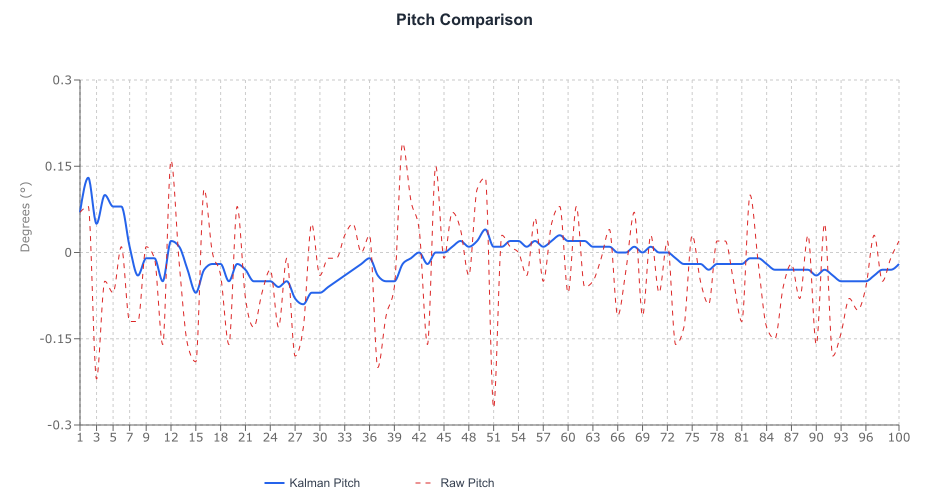
\includegraphics[width=0.8\textwidth]{images/kalman_comparison_pitch_2025-06-23.png}
    \caption{Pitch: Vergleich Rohdaten und Kalman-Filter}
    \label{fig:pitch_pitch}
    \end{figure}

    \begin{figure}[H]
        \centering
        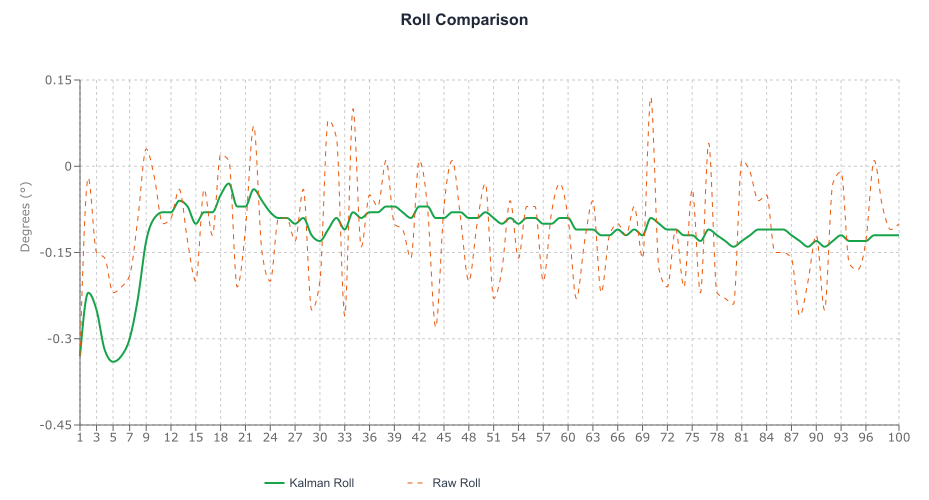
\includegraphics[width=0.8\textwidth]{images/kalman_comparison_roll_2025-06-23.png}
        \caption{Roll: Vergleich Rohdaten und Kalman-Filter}
        \label{fig:roll_roll}
    \end{figure}
\end{samepage}


